%!TEX root = /Users/louis/Documents/PhD/Deliverables/Thesis/thesis.tex

\section{Quantitive Comparison of Model Migration Languages}
\label{sec:quantitive}
In Section~\ref{sec:requirements_identification}, the following research requirement was identified: \emph{This thesis must implement and evaluate a domain-specific language for specifying and executing model migration strategies, comparing it to existing languages for specifying model migration strategies.} As discussed in Section~\ref{sec:flock}, this thesis contributes Epsilon Flock, a domain-specific language for model migration. This section approches the second part of the above research requirement by comparing Flock with languages that are used in contemporary migration tools. 

In developer-driven migration, a programming language codifies the migration strategy. Because migration involves deriving the migrated model from the original, migration strategies typically access information from the original model and, based on that information, update the migrated model in some way. As such, migration is written in a language with constructs for accessing and updating the original and migrated models. Here, those language constructs are termed \textit{model operations}. Using examples of co-evolution, this section explores the variation in frequency of model operation over different model migration languages, and discusses to what extent the results of this comparison can be used to assess the suitability of the languages considered for model migration.

As discussed in Chapter~\ref{Implementation}, the languages currently used for model migration vary. Model-to-model transformation languages are used in some migration tools (e.g. \cite{cicchetti08automating,garces09managing}), and general-purpose languages in others (e.g. \cite{herrmannsdoerfer09cope,hussey06advanced}). Irrespective of the language used for migration, the way in which a migration tool relates original and migrated model elements falls into one of two categories: new- or existing-target, which were first introduced in Section~\ref{subsec:existing_migration_languages}. In the former, the migrated model is created afresh by the execution of the migration strategy. In the latter, the migrated model is initialised as a copy of the original model and then the migration strategy is executed.

Flock contributes a novel approach for relating original and migrated model elements, termed conservative copy. Conservative copy is a hybrid of new- and existing-target approaches. This section compares new-target, existing-target and conservative copy in the context of model migration. Section~\ref{subsubsec:quantitive_data} describes the data used in the comparison. The method for the comparison is discussed in Section~\ref{subsubsec:quantitive_method}. Section~\ref{subsubsec:quantitive_model_operations} identifies model operations for each of the migration languages used in the comparison, and Section~\ref{subsubsec:quantitive_results} presents and analysis the results.

\subsection{Data}
\label{subsubsec:quantitive_data}
Five examples of co-evolution were used to compare new-target, existing-target and conservative copy. This section briefly discusses the data used in the comparison.

\subsubsection{Co-evolution Examples}
To remove one of the possible threats to the validity of the comparison, the examples used were distinct from those used to identify the thesis requirements in Chapter~\ref{Analysis}. The five examples used in this section are taken from three projects.

Two examples were taken from the \emph{Newsgroup} project, which performs statistical analysis of NNTP newsgroups and was developed by Dimitris Kolovos, a lecturer in this department. One example was taken from \emph{UML} (the Unified Modeling Language), an OMG specification of a language for modelling software systems. Two examples were taken from \emph{GMF} (Graphical Modeling Framework) \cite{gronback09emp}, an Eclipse project for generating graphical model editors.

\subsubsection{Selection of Migration Languages}
As discussed above, there are two ways in which existing migration languages relate original and migrated model elements, new- and existing-target. Flock contributes a third way, conservative copy. For the comparison with Flock, one new- and one existing-target language was chosen.

The Atlas Transformation Language (ATL), a model-to-model transformation language that has been used in \cite{cicchetti08automating,garces09managing} for model migration. As discussed in Section~\ref{subsec:existing_migration_languages}, model-to-model transformation languages support only new-target transformations for model migration\footnote{Because, in model migration, the source and target metamodels are not the same.}.

The author is aware of two approaches to migration that use existing-target transformations. In COPE \cite{herrmannsdoerfer09cope}, migration strategies can be hand-written in Groovy when no co-evolutionary operator is applicable. As discussed in Section~\ref{subsec:existing_migration_languages}, COPE's Groovy migration strategies use an existing-target approach. COPE provides six functions for interacting with model elements, such as \texttt{set}, for changing the value of a feature, and \texttt{unset}, for removing all values from a feature. In the remainder of this section, the term \emph{Groovy-for-COPE} is used to refer to the combination of the Groovy programming language and the functions provided by COPE for use in hand-written migration strategies. In Ecore2Ecore \cite{hussey06advanced}, migration is performed when the original model is loaded, effectively an existing-target approach.

The comparison to Flock described in this section uses ATL to represent new-target approaches and Groovy-for-COPE to represent existing-target approaches. Groovy-for-COPE was preferred to Ecore2Ecore because the latter is not as expressive\footnote{Communication with Ed Merks, Eclipse Modeling Project leader, 2009, available at \url{http://www.eclipse.org/forums/index.php?t=tree&goto=486690&S=b1fdb2853760c9ce6b6b48d3a01b9aac}} and cannot be used for migration in the co-evolution examples considered here.

\subsection{Method}
\label{subsubsec:quantitive_method}
For each example of co-evolution, a migration strategy was written using each migration language (ATL, Groovy-for-COPE and Flock). The co-evolution examples considered included reference migrated models. The correctness of each migration strategy was assured by comparing the migrated model produced with the corresponding reference migrated model.

Next, a set of model operations were identified, as described in Section~\ref{subsubsec:quantitive_model_operations} and a program was written to count the frequency of each model operation in each migration strategy. The counting program was tested by comparison to manual counts.

The method described above introduces one non-trivial threat to the validity of the comparison. Because the author is obviously more familiar with Flock than with ATL and Groovy-for-COPE, it is possible that the migration strategies written in the latter two languages may contain more model operations than necessary. In some cases, it was possible to reduce the effects of this threat by re-using or adapting existing migration strategy code written by the migration language authors. This is discussed further in the sequel.

\subsection{Model Operations}
\label{subsubsec:quantitive_model_operations}
The way in which model operations were counted is now described. Two categories of model operation were considered: copying and deleting. Copying (deleting) operations are used to assign (remove) values to (from) elements of the migrated model. The three languages considered use different syntax for semantically equivalent statements. Some of the languages provide more than one construct for copying or deleting values. The remainder of this section lists the concrete syntax of the model operations in each language. In addition, the extent to which the comparison described in this section was able to use code written by the authors of each language is discussed.

\subsubsection{Atlas Transformation Language (ATL)}
For the Atlas Transformation Language (ATL), the following model operations were counted:
	
\begin{itemize}
	\item \textbf{Copying:} Assignment to a feature:
	\subitem \texttt{<feature> <- <value>} 
\end{itemize}

Deleting operations are not used in new-target migration strategies. A new-target migration strategy specifies only those values that must appear in the migrated model and, unlike existing-target approaches and conservative copy, no values are copied automatically prior to the execution of the migration.


\subsubsection{Groovy-for-COPE}
For Groovy-for-COPE, the following model operations were counted:

\begin{itemize}
	\item \textbf{Copying:} Assignment to a feature:
	\subitem \texttt{<element>.<feature> = <value>}
	\subitem \texttt{<element>.<feature>.add(<value>)}
	\subitem \texttt{<element>.<feature>.addAll(<collection\_of\_values>)}
	\subitem \texttt{<element>.set(<feature>) = <value>}
	
	\item \textbf{Deleting:} Unsetting a feature:
	\subitem \texttt{<element>.<feature>.unset()}	
	
	\item \textbf{Deleting:} Removing a model element:
	\subitem \texttt{delete <element>}
\end{itemize}

Groovy-for-COPE provides four assignment statements. The first is typical. The second and third are used to add values to a collection. The fourth is used for reflective access to a model.

The deleting operations are necessary for some existing-target migration strategies, because the migrated model (which is initialised as a copy of the original model) may contain data that is no longer captured in the evolved metamodel.

As discussed in Section~\ref{subsec:co-evolution_categorisation}, COPE provides a library of built-in, reusable co-evolutionary operators. Each co-evolutionary operator specifies a metamodel evolution along with a corresponding model migration strategy. To mitigate the chance that the author, who is less familiar with COPE than Flock, introduced additional model operations, writing the Groovy-for-COPE migration strategies involved, where possible, applying an appropriate COPE co-evolutionary operator and counting the number of model operations in the generated migration strategy. Not all of the examples considered could be specified using co-evolutionary operators, and, in these cases, the Groovy-for-COPE migration strategy was written entirely by the author.


\subsubsection{Epsilon Flock}
Epsilon Flock, a transformation language tailored for model migration, was developed in this thesis and discussed in Chapter~\ref{Implementation}. Flock uses the Epsilon Object Language (EOL) \cite{kolovos06eol} to access and update model values. For Flock, the following model operations were counted:

\begin{itemize}
	\item \textbf{Copying:} Assignment to a feature:
	\subitem \texttt{<element>.<feature> := <value>} 
	\subitem \texttt{<element>.<feature>.add(<value>)}
	\subitem \texttt{<element>.<feature>.addAll(<collection\_of\_values>)}
	
	\item \textbf{Deleting:} Removing a model element:
	\subitem \texttt{delete <element>}
\end{itemize}

Like Groovy-for-COPE, Flock provides several assignment statements. The first is typical. The second and third are used to add values to a collection.

Flock provides a remove operation but not an unset. The former is required to remove model elements that no longer conform to the target metamodel. Flock does not provide an unset operation because the conservative copy algorithm will never copy to the migrated model any value that does not conform to the evolved metamodel. 


\subsection{Results}
\label{subsubsec:quantitive_results}
By measuring the number of model operations in model migration strategies, the way in which each co-evolution approach relates original and migrated model elements was investigated. The five examples of model migration discussed above were measured to obtain the results shown in Table~\ref{tab:model_operations_results}.

In addition, the results from measuring the examples identified from Chapter~\ref{Analysis} are shown in Table~\ref{tab:model_operations_results_analysis_examples}. However, because the examples used to produce the measurements shown in Table~\ref{tab:model_operations_results_analysis_examples} were used to design Flock, the measurements in Table~\ref{tab:model_operations_results_analysis_examples} are less relevant to the evaluation presented here than the measurements shown in Table~\ref{tab:model_operations_results}. Nevertheless, the measurements made in Table~\ref{tab:model_operations_results_analysis_examples} are included in the interest of transparency.

\begin{table}
	\centering
	\begin{tabular}{|r|c|c|c|}
		\hline
		                              & \multicolumn{3}{|c|}{\textbf{Migration Language}} \\
													  			& \multicolumn{3}{|c|}{Source-Target Relationship} \\
		\hline
		                              & \textbf{ATL} & \textbf{G-f-C} & \textbf{Flock} \\
		(Project) Example             & New & Existing & Conservative \\
		\hline
		\hline
		(Newsgroup) Extract Person    & 9  &  6  &  5  \\
		\hline                       
		(Newsgroup) Resolve Replies   &  8  &  3  &  2  \\
		\hline                       
		(UML) Activity Diagrams       &  15  &  15  &  8  \\
		\hline                       
		(GMF) Graph                   &  101  &  11  &  14  \\
		\hline                       
		(GMF) Gen2009                 &  310  &  16  &  16  \\
		\hline
	\end{tabular}
	\caption{Model operation frequency (evaluation examples).}
	\label{tab:model_operations_results}
\end{table}

\begin{table}
	\centering
	\begin{tabular}{|r|c|c|c|}
		\hline
		                              & \multicolumn{3}{|c|}{\textbf{Migration Language}} \\
													  			& \multicolumn{3}{|c|}{Source-Target Relationship} \\
		\hline
		                              & \textbf{ATL} & \textbf{G-f-C} & \textbf{Flock} \\
		(Project) Example             & New & Existing & Conservative \\
		\hline
		\hline
		(FPTC) Connections            & 6  & 6   & 3  \\
		\hline
		(FPTC) Fault Sets             & 7  & 5   & 3  \\
		\hline
		(GADIN) Enum to Classes       & 4  & 1   & 0  \\
		\hline
		(GADIN) Partition Cont        & 5  & 3   & 2  \\
		\hline
		(Literature) PetriNets        & 12  & 10   & 6  \\
		\hline
		(Newsgroup) Extract Person    & 9  & 6   & 5  \\
		\hline
		(Newsgroup) Resolve Replies   & 8  & 3   & 2  \\
		\hline
		(Process-Oriented) Split CP   & 8  & 1   & 1  \\
		\hline
		(Refactor) Cont to Ref        & 4  & 5   & 3  \\
		\hline
		(Refactor) Ref to Cont        & 3  & 4   & 3  \\
		\hline
		(Refactor) Extract Class      & 5  & 4   & 2  \\
		\hline
		(Refactor) Extract Subclass   & 6  & 0   & 0  \\
		\hline
		(Refactor) Inline Class       & 4  & 5   & 2  \\
		\hline
		(Refactor) Move Feature       & 6  & 2   & 1  \\
		\hline
		(Refactor) Push Down Feature  & 6  & 0 & 0  \\
		\hline
	\end{tabular}
	\caption{Model operation frequency (analysis examples).}
	\label{tab:model_operations_results_analysis_examples}
\end{table}

For four of the five examples in Table~\ref{tab:model_operations_results}, conservative copy requires less model operations than new-target and existing-target. The GMF Graph example is the exception to this trend.

For all of the five examples in Table~\ref{tab:model_operations_results}, no migration strategy specified with existing-target contained less model operations when encoded with new-target. However, three of the Refactor examples in Table~\ref{tab:model_operations_results_analysis_examples} do not follow this trend.

The results are now investigated, starting by discussing the differences between the source-target relationships. Investigating the results led to the discovery of two limitations of the conservative copy implementation in Flock, relating to sub-typing and side-effects during initialisation. These limitations are also discussed below.

\subsubsection{Source-Target Relationships}
New-target, existing-target and conservative copy initialise the migrated model in a different way. New-target initialises an empty model, while existing-target initialises a complete copy of the original model. Conservative copy initialises the migrated model by copying only those model elements from the original model that conform to the migrated metamodel.

New- and existing-target are opposites. In the former, explicit assignment operations must be used to copy values from original to migrated model for each feature that is not affected by the metamodel evolution. By contrast, in the latter unset operations must be used when the value of a feature should not have been copied.

In situations where a large number of metamodel features have not been affected by evolution, expressing migration with a new-target transformation language requires more model operations than using an existing-target transformation language. This is particularly noticeable in the GMF examples shown in Table~\ref{tab:model_operations_results}, where ATL (new-target) requires many more model operations than Groovy-for-COPE (existing-target) and Flock (conservative copy).

In situations where a large number of metamodel features have been renamed, expressing migration with an existing-target transformation language requires more model operations than using a new-target transformation language. This is because, in an existing-target transformation language, two model operations (an unset and an assignment) are needed to migrate values in response to the renaming of a feature:

\texttt{<element>.<newFeature> = <element>.unset(<oldFeature>)}

By contrast, a new-target transformation language requires only one model operation (an assignment):

\texttt{<migrated\_element>.<feature> = <original\_element>.<feature>}

The UML (Table~\ref{tab:model_operations_results}) and Refactor Inline Class (Table~\ref{tab:model_operations_results_analysis_examples}) examples contained several feature renamings, and consequently the Groovy-for-COPE (existing-target) figure was nearer to the ATL (new-target) figure than the Flock (conservative copy) figure. This is contrary to the trend in Tables~\ref{tab:model_operations_results} and \ref{tab:model_operations_results_analysis_examples}.

Conservative copy is a hybrid of new- and existing target. Model values that have been affected by evolution are not copied to the migrated model, and so the migration strategy need not unset affected model values. Model values that have not been affected by evolution are copied to the migrated model, and so the migration strategy need not explicitly copy unaffected model values.

Two conclusions can be drawn from this discussion. Firstly, in general, less model operations are used when specifying a migration strategy with a conservative copy migration language than when specifying the same migration strategy with a new- or existing-target migration language.

Secondly, in the examples studied here, there are often more features unaffected by metamodel evolution than affected. Consequently, specifying model migration with a new-target migration language requires more model operations than in an existing-target migration language for the examples shown in Tables~\ref{tab:model_operations_results} and ~\ref{tab:model_operations_results_analysis_examples}. \cite{sprinkle03thesis} proposes that metamodel evolution often involves changes to relatively few metamodel elements, and the results presented in this section support his argument.  

\subsubsection{Subtyping}
Form the GMF Graph example (Table~\ref{tab:model_operations_results}), conservative copy requires more model operations than existing-target. Investigation of this result revealed a limitation in conservative copy limitation in Flock, which is now described.

Figure~\ref{fig:subtyping} shows a simplified part of the GMF Graph metamodel prior to evolution. When the metamodel evolved, the types of the \texttt{figure} and \texttt{accessor} features were changed. Consequently, the migration strategy needed to change the values stored in the \texttt{figure} and \texttt{accessor} features. In the simplified example presented here, the types of the \texttt{figure} and \texttt{accessor} features were changed from string to integer. The intended migration semantics are for the integer value to be the length of the original string value. This is a simplification that is representative of the actual GMF Graph metamodel evolution.

\begin{figure}[htbp]
  \centering
  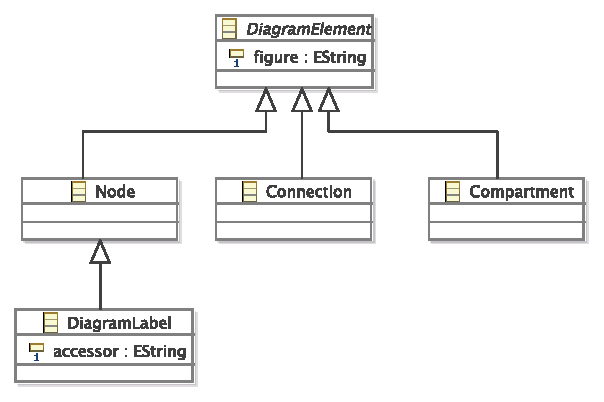
\includegraphics[scale=0.75]{6.Evaluation/images/subtyping.pdf}
  \caption{Simplified fragment of the GMF Graph metamodel.}
  \label{fig:subtyping}
\end{figure}

In ATL, the migration strategy for the metamodel evolution discussed above can be expressed using two model operations, because an ATL transformation rule may inherit the body of another. The \texttt{DiagramElements} rule on lines 1-4 of Listing~\ref{lst:graph_atl} specifies that the value of the figure feature should be the length of the original value. For \texttt{Node}s, \texttt{Connection}s and \texttt{Compartment}s, migration can be specified simply by extending the \texttt{DiagramElements} rule (lines 6-19). For \texttt{DiagramLabel}s, the values of both the accessor and figure feature must be migrated. On lines 21-24, the \texttt{DiagramLabels} extends \texttt{Nodes} and hence \texttt{DiagramElements} to inherit the body of the latter for migrating figures, and, in addition, the \texttt{DiagramLabels} rule defines the migration for the value of the \texttt{accessor} feature.

\begin{lstlisting}[basicstyle=\ttfamily\footnotesize, flexiblecolumns=true, numbers=left, nolol=true, caption=Simplified GMF Graph model migration in ATL, label=lst:graph_atl, language=ATL, tabsize=2]
abstract rule DiagramElements {
	from o : Before!DiagramElement
	to   m : After!DiagramElement ( figure <- o.figure.length()	)
}

rule Nodes extends DiagramElements {
	from o : Before!Node
	to   m : After!Node
}

rule Connections extends DiagramElements {
	from o : Before!Connection
	to   m : After!Connection
}

rule Compartments extends DiagramElements {
	from o : Before!Compartment
	to   m : After!Compartment
}

rule DiagramLabels extends Nodes {
	from o : Before!DiagramLabel
	to   m : After!DiagramLabel (	accessor <- o.accessor.length()	)
}
\end{lstlisting}

In Groovy-for-COPE, the migration is similar to ATL. However, Groovy-for-COPE is entirely imperative, and so the migration (Listing~\ref{lst:graph_cope}) is more concise than the ATL migration (Listing~\ref{lst:graph_atl}). In Listing~\ref{lst:graph_cope}, a loop iterates over each instance of \texttt{DiagramElement} (line 1), migrating the value of its figure feature (line 2). If the \texttt{DiagramElement} is also a \texttt{DiagramLabel} (line 4), the value of its accessor feature is also migrated (line 5).

\begin{lstlisting}[basicstyle=\ttfamily\footnotesize, flexiblecolumns=true, numbers=left, nolol=true, caption=Simplified GMF Graph model migration in COPE, label=lst:graph_cope, language=COPE, tabsize=2]
for (diagramElement in subtyping.DiagramElement.allInstances()) {
	diagramElement.figure = diagramElement.figure.length()
	
	if (subtyping.DiagramLabel.allInstances.contains(diagramElement)) {
		diagramElement.accessor = diagramElement.accessor.length()
	}
}
\end{lstlisting}

In both ATL and Groovy-for-COPE, only 2 model operations are required for this migration: an assignment for each of the two features being migrated. However, the equivalent Flock migration strategy, shown in Listing~\ref{lst:graph_flock}, requires 5 model operations. In Flock, a migrate rule must be specified for each concrete subtype of \texttt{DiagramElement}. A single \texttt{DiagramElement} rule cannot be used to migrate the concrete subtypes because, when a rule does not specify a \texttt{to} part, Flock will create an instance of the type named after the \texttt{migrate} keyword (i.e. \texttt{DiagramElement} here). Because \texttt{DiagramElement} is abstract, Flock will fail with a runtime error. Furthermore, because only one rule can be applied to each original model element, the \texttt{DiagramLabel} rule (lines 9-12) must migrate the values of both the figure and accessor features, and cannot exploit the kind of re-use provided by ATL with rule inheritance.

\begin{lstlisting}[basicstyle=\ttfamily\footnotesize, flexiblecolumns=true, numbers=left, nolol=true, caption=Simplified GMF Graph model migration in Flock, label=lst:graph_flock, language=Flock, tabsize=2]
migrate Compartment {
	migrated.figure := original.figure.length();
}

migrate Connection {
	migrated.figure := original.figure.length();
}

migrate DiagramLabel {
	migrated.figure   := original.figure.length();
	migrated.accessor := original.accessor.length();
}

migrate Node {
	migrated.figure := original.figure.length();
}
\end{lstlisting}

The example presented in this section highlights a limitation of the conservative copy algorithm as it is implemented in Flock. The extent to which this limitation can be addressed with changes to the implementation of Flock, and in general, is discussed in Section~\ref{sec:future_work}. This section now considers one further limitation of existing-target and conservative copy migration languages.

\subsubsection{Side-Effects during Initialisation}
The measurements observed for one of the examples of co-evolution from Chapter~\ref{Analysis}, Change Reference to Containment, cannot be explained by the conceptual differences between source-target relationship. Instead, the way in which the source-target relationship is implemented must be considered.

When a reference feature is changed to a containment reference during metamodel evolution, constructing the migrated model by starting from the original model (as is the case with existing-target and conservative copy) can have side-effects which complicate migration.

In the Change Reference to Containment example, a \texttt{System} initially comprises \texttt{Port}s and \texttt{Signature}s (Figure~\ref{fig:ref2cont_original_mm}). A \texttt{Signature} references any number of \texttt{ports}. The metamodel is to be evolved so that \texttt{Port}s can no longer be shared between \texttt{Signature}s.

\begin{figure}[htbp]
  \centering
  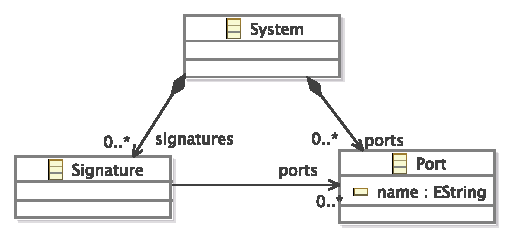
\includegraphics[scale=0.75]{6.Evaluation/images/change_ref_to_cont_before.pdf}
  \caption{Original metamodel.}
  \label{fig:ref2cont_original_mm}
\end{figure}

The evolved metamodel is shown in Figure~\ref{fig:ref2cont_evolved_mm}. \texttt{Signature}s now contain - rather than reference - \texttt{Port}s. Consequently, the \texttt{ports} feature of \texttt{System} is no longer required and is removed.

\begin{figure}[htbp]
  \centering
  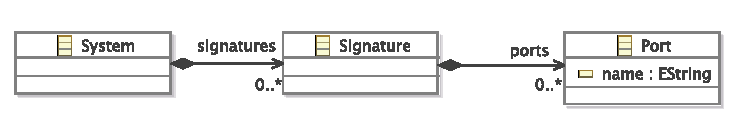
\includegraphics[scale=0.75]{6.Evaluation/images/change_ref_to_cont_after.pdf}
  \caption{Evolved metamodel.}
  \label{fig:ref2cont_evolved_mm}
\end{figure}

The migration strategy is straightforward in a new-target migration language: for each \texttt{Signature} in the original model, each member of the \texttt{ports} feature is cloned and added to the \texttt{ports} feature of the equivalent \texttt{Signature}.

\begin{lstlisting}[basicstyle=\ttfamily\footnotesize, flexiblecolumns=true, numbers=left, nolol=true, caption=Change R to C model migration in ATL, label=lst:ref2cont_atl, language=ATL, tabsize=2]
rule Systems {
	from
		o : Before!System
	to
		m : After!System ( signatures <- o.signatures )
}

rule Signature {
	from
		o : Before!Signature
	to
		m : After!Signature (
			ports <- o.ports->collect(p | thisModule.Port(p))
		)
}

lazy rule Port {
	from
		o : Before!Port
	to
		m : After!Port ( name <- o.name )
\end{lstlisting}

In existing-target and conservative copy migration languages, migration is less straightforward because the value of a containment reference (\texttt{Signature\#ports}) is set automatically by the migration strategy execution engine. When a containment reference is set, the contained objects are removed from their previous containment reference (i.e. setting a containment reference can have side-effects). Therefore, in a \texttt{System} where more than one \texttt{Signature} references the same \texttt{Port}, the migrated model cannot be formed by copying the contents of \texttt{Signature\#ports} from the original model. Attempting to do so causes each \texttt{Port} to be contained only in the last referencing \texttt{Signature} that was copied.

In COPE, conformance is checked only after execution of the migration strategy, when the model is transformed to a metamodel-specific representation. Therefore, the containment nature of the reference is not enforced until after the migration strategy is executed. Hence, the migration strategy discussed here can be specified by unsetting the contents of the \texttt{ports} reference (line 4 of Listing~\ref{lst:ref2cont_cope}), and creating a copy of each referenced \texttt{Port} (lines 5-7 of Listing~\ref{lst:ref2cont_cope}).

Unlike the ATL migration strategy, the ports in the Groovy-for-COPE migration strategy are cloned in the same model as the original port. Consequently, the Groovy-for-COPE migration strategy must either only clone ports that are referenced by more than one signature or clone every referenced port, but delete all of the original ports. The latter approach requires 2 more model operations (to populate and delete the original ports) than the former (shown in Listing~\ref{lst:ref2cont_cope}).

\begin{lstlisting}[basicstyle=\ttfamily\footnotesize, flexiblecolumns=true, numbers=left, nolol=true, caption=Change R to C model migration in COPE, label=lst:ref2cont_cope, language=COPE, tabsize=2]
def contained = []

for(signature in refactorings_changeRefToCont.Signature.allInstances) {
  for(port in signature.ports)) {
	  // when more than one Signature references this port
	  if (contained.contains(port)) {
      def clone = Port.newInstance()
      clone.name = port.name
      signature.ports.add(clone)
      signature.ports.remove(port)
		} else {
			contained.add(port)
		}
  }
}

for(port in refactorings_changeRefToCont.Port.allInstances) {
	if (not refactorings_changeRefToCont.Signature.allInstances.any { it.ports.contains(port) }) {
	  	port.delete()
	}
}
\end{lstlisting}

In Flock, the containment nature of the reference is enforced when the migrated model is initialised. Because changing the contents of a containment reference can have side-effects, a \texttt{Port} that appears in the \texttt{ports} reference of a \texttt{Signature} in the original model may not have been automatically copied to the \texttt{ports} reference of the equivalent \texttt{Signature} in the migrated model during initialisation. Consequently, the migration strategy must check the \texttt{ports} reference of each migrated \texttt{Signature}, cloning only those \texttt{Port}s that have not be automatically copied during initialisation (see line 3 of Listing~\ref{lst:ref2cont_flock}).

\begin{lstlisting}[basicstyle=\ttfamily\footnotesize, flexiblecolumns=true, numbers=left, nolol=true, caption=Change R to C model migration in Flock, label=lst:ref2cont_flock, language=Flock, tabsize=2]
migrate Signature {
	for (port in original.ports) {
		if (migrated.ports.excludes(port.equivalent())) {
			var clone := new Migrated!Port;
			clone.name := port.name;
			migrated.ports.add(clone);
		}
	}
}

delete Port when: not Original!Signature.all.exists(s|s.ports.includes(original))
\end{lstlisting}

The Groovy-for-COPE and Flock migration strategies must also remove any \texttt{Port}s which are not referenced by any \texttt{Signature} (lines 17-21 of Listing~\ref{lst:ref2cont_cope}, and line 11 of Listing~\ref{lst:ref2cont_flock} respectively), whereas the ATL migration strategy, which initialises any empty migrated model, does not copy unreferenced \texttt{Port}s.

When a non-containment reference is changed to a containment reference, producing a migration strategy in Flock and Groovy-for-COPE requires the user to be aware of the side-effects that can occur during initialisation. It may be possible to extend the existing-target and conservative copy algorithms used in COPE and Flock to automatically perform cloning when a reference is changed to be a containment reference. This is discussed further in Section~\ref{sec:future_work}.


\subsection{Summary}
By measuring frequency of model operations, this section has compared, in the context of model migration, three approaches to relating source-target relationship: new-target, existing-target and conservative copy. The results have been analysed and the measurement method described.

The analysis of the measurements has shown that new- and existing-target migration languages are better suited to different contexts. New-target languages require less model operations than existing-target languages when metamodel evolution involves the renaming of features. Existing-target languages require less model operations than new-target languages when metamodel evolution does not affect most model elements. For the examples considered here, the latter context was more common. Conservative copy requires less model operations than both new- and existing-target in almost all of the examples considered here.

The comparison has highlighted two limitations of the conservative copy algorithm implemented in Epsilon Flock, and this section has shown how these limitations are problematic for specifying some types of migration strategy. 

The author is not aware of any existing quantitive comparisons of migration languages, and, as such, the best practices for conducting such comparisons are not clear. The method used in obtaining these measurements has been described to provide a foundation for future comparisons. 
